%% Template for MLP Coursework 4

%% Based on  LaTeX template for ICML 2017 - example_paper.tex at 
%%  https://2017.icml.cc/Conferences/2017/StyleAuthorInstructions

\documentclass{article}
\usepackage[T1]{fontenc}
\usepackage{amssymb,amsmath}
\usepackage{txfonts}
\usepackage{microtype}
\usepackage{xspace}
\xspaceaddexceptions{\%}

% Lists with less spacoing between items
\usepackage{paralist}

% For figures
\usepackage{graphicx}
\usepackage{subfig} 

% For citations
\usepackage{natbib}

% For algorithms
\usepackage{algorithm}
\usepackage{algorithmic}

% the hyperref package is used to produce hyperlinks in the
% resulting PDF.  If this breaks your system, please commend out the
% following usepackage line and replace \usepackage{mlp2017} with
% \usepackage[nohyperref]{mlp2017} below.
\usepackage[hyphen]{url}
\urlstyle{same}
\usepackage{hyperref}
\usepackage{comment}
\usepackage{titlesec}
\usepackage{svg}
\usepackage{caption}
\captionsetup[table*]{width=0.9\textwidth}

% Packages hyperref and algorithmic misbehave sometimes.  We can fix
% this with the following command.
\newcommand{\theHalgorithm}{\arabic{algorithm}}


% Set up MLP coursework style (based on ICML style)
\usepackage{mlp2022}
\mlptitlerunning{MLP Coursework 4 -- Final Report (\groupNumber)}
\bibliographystyle{icml2017}
\setlength{\bibsep}{10pt}


\DeclareMathOperator{\softmax}{softmax}
\DeclareMathOperator{\sigmoid}{sigmoid}
\DeclareMathOperator{\sgn}{sgn}
\DeclareMathOperator{\relu}{relu}
\DeclareMathOperator{\lrelu}{lrelu}
\DeclareMathOperator{\elu}{elu}
\DeclareMathOperator{\selu}{selu}
\DeclareMathOperator{\maxout}{maxout}


\titlespacing{\section}{-1pt}{\parskip}{-\parskip}




%% You probably do not need to change anything above this comment

%% REPLACE this with your project title, group ID and list of student numbers for the group
%\def\projectTitle{Title}
\def\groupNumber{G060}
\def\studentNumbers{s2446690, s2305829, s2420055}

\begin{document} 
\twocolumn[
\mlptitle{Enhancing Video Description Generation with Deep Learning and ChatGPT: A Comparative Study}

\centerline{\groupNumber\ (\studentNumbers)}

\vskip 7mm
]

\begin{abstract} 
This study aims to tackle the challenging task of generating semantically meaningful video descriptions using deep learning techniques. Our baseline model uses a simple combination of an image feature extraction CNN and vanilla transformer. We compare its performance with 4 state-of-the-art end-to-end video captioning models, including PDVC, MART, DenseCap, and SwinBERT, on the ActivityNet dataset. The coherency and comprehensibility of the descriptions generated are enhanced utilising ChatGPT, a new GPT-3 based LLM. We evaluate our models using metrics such as METEOR, SARI, ROUGE, and Cross-Encoders on 26 videos. Among all the models tested, SwinBERT and DenseCap exhibited the best average similarity scores of $\approx$ 0.25.
\end{abstract} 

\section{Introduction}
\label{sec:intro}
% Video captioning models have become increasingly important in today's digital age. As video content continues to proliferate across various platforms, the need for accessible and engaging captions has never been more critical. These models provide a way for people with hearing disabilities or those who prefer to consume content with captions to access video content. \cite{intro1} Additionally, they can be used to translate captions into multiple languages, improving the reach of video content across the globe. \cite{intro2} Furthermore, video captioning models can enhance the user experience of video content by providing text that can be followed along with the audio. In this paper, we will explore the various reasons why video captioning models are crucial and how they have impacted the world of digital content.

% The aim of this research project is to improve the efficiency of video consumption by presenting the most salient and relevant information in a concise and understandable format. The motivation for this study comes from the automatic chapter generation feature in YouTube, which allows users to navigate long videos more easily and locate important segments. Specifically, we will investigate how to automatically identify and summarize the key parts of a video, such as the main topics, concepts, and events, using natural language processing and machine learning techniques. By doing so, we hope to reduce the time and effort required for users to comprehend large or lengthy videos, especially in educational contexts where video lectures or tutorials can last for hours.

% The purpose of video description generation, also known as video captioning, is to automatically generate captions for videos by understanding the action and events in the video, which can help in the retrieval of the video efficiently through text \cite{intro4}. Video captioning is a challenging task due to the complexity and diversity of video content, and it requires understanding the temporal relationship between video frames \cite{intro3}. The automatic generation of video descriptions can be useful in many aspects, including helping visually impaired individuals to understand the content of videos. With the incomparable performance of deep learning in the field of computer vision and natural language processing, research in this field has been exponentially increasing throughout the past decades \cite{intro2}. Therefore, developing accurate video captioning models is crucial for various applications such as video indexing and retrieval.

Video captioning models \cite{Aafaq2019SpatioTemporalDA,Chen2019DeepLF, Liu2018SibNetSC,Pei2019MemoryAttendedRN,Shi2020LearningSC} play a critical role in providing captions for video content that are both accessible and engaging. This is particularly important for individuals with hearing impairments or those who prefer closed captions \cite{intro1}. The automatic generation of video descriptions can also help visually impaired individuals to understand the content of videos \cite{intro4}. By translating captions into multiple languages, these models can also help increase the reach of video content around the world \cite{intro2}. Moreover, video captioning models can enhance a user's viewing experience by providing text that can be followed along with the audio. However, video captioning continues to remain a challenging task as it requires understanding the temporal relationship between video frames \cite{intro2}. Developing accurate video captioning models is thus crucial for various other applications such as video indexing and retrieval.

Our research focuses on leveraging natural language processing and deep learning methods to automatically identify and summarise significant elements of a video, such as its primary topics, concepts, and events. This can help reduce the time and effort required for users to comprehend large or lengthy videos, especially in educational contexts where video lectures or tutorials can last for hours. For example, the automatic chapter generation feature in YouTube allows users to navigate long videos more easily and locate important segments. In contrast to generating video summaries or highlights, our objective is to generate video descriptions that concisely capture the essence of the content, thereby enhancing accessibility and comprehension for a broader audience.

\section{Related work}
\label{sec:relwork}
Video captioning has been extensively studied in recent years, with various approaches proposed such as using convolutional neural networks (CNNs) and recurrent neural networks (RNNs) for content encoding and decoding \cite{yu2016video}. Initial methods involved encoding video frames into a fixed-length vector via CNNs and subsequently decoding it into a natural language sentence with RNNs \cite{pan2016hierarchical}. Attention mechanisms have also been introduced to improve the performance of these models by focusing on they key regions of videos \cite{zhou2018end}. Transfer learning techniques have also been applied to improve the efficiency of video captioning models by pre-training them on large-scale image or video datasets \cite{mahajan2018exploring}. More recent studies have explored the use of transformer-based architectures, such as the popular BERT model, for video captioning tasks \cite{kim2020dense}. Transformer-based models involve understanding and modeling spatial-temporal dynamics in videos and generating output sequences of words. These models learn from offline extracted video representations using feature extractors trained on image/video understanding tasks to extract appearance (2D) and motion features (3D) from densely sampled video frames \cite{Lei2021LessIM,Luo2020UniViLMAU}. However, end-to-end training with this approach is computationally intensive. In addition, some research has focused on temporal event proposal such as boundary-based methods that use salient frames to create proposals for identifying event-containing segments in untrimmed videos. However, these methods rely on binary mask vectors and scalar descriptiveness scores that are not informative enough to guide feature representation \cite{Li2018JointlyLA,Singh2022V2TVT}.

\section{Data set and task} 
\subsection{Datasets}
Flickr8k is a widely used benchmark dataset for image captioning, containing 8,000 images and 40,000 captions \cite{hodosh2013framing}. Each image in the dataset is accompanied by five captions written by different annotators, which ensures a diversity of descriptions for each image. The dataset was initially designed to assess the effectiveness of image captioning models and has since been widely adopted in research for exploring and contrasting various image captioning techniques. This dataset is the foundation of our baseline model.

ActivityNet is a benchmark dataset for human activity understanding that contains 19,994 untrimmed videos from 203 activity classes \cite{activitynet}. It is divided into training, validation, and testing subsets and includes 849 hours of videos in total. It is the largest dataset for temporal activity detection and features a hierarchical annotation framework and multiple modalities for multi-modal learning and fusion. The main purpose of ActivityNet is to provide a standard reference for evaluating algorithms that aim to comprehend human activities and creating video captioning models.

\subsection{Task}
At a broad level, our study performs a comprehensive 5-way comparison of video description models on the ActivityNet dataset. In particular, we compare our crude baseline model for video description generation with 4 advanced transformer-based end-to-end models, namely, DenseCap \cite{johnson2016densecap}, MART \cite{liu2020mobile}, PDVC \cite{le2021pdvc}, and SwinBERT \cite{lin2022swinbert}. ChatGPT is a large language model developed by OpenAI, based on the GPT-3 architecture \cite{Brown2020LanguageMA}. It uses deep neural networks to generate human-like responses to natural language input. The output video descriptions from each model are passed through ChatGPT to improve their quality and fluency. This serves as our new benchmark for performance evaluation. The goal is to identify the most effective method for producing high-quality video summaries that are coherent and semantically meaningful. 

The subsequent sections of this report cover the methodologies, experiments conducted, and metrics used to evaluate the results.

\section{Methodology}
\subsection{Baseline}
Dense video captioning is a challenging task that involves both event localisation and event captioning. The two subtasks are typically solved in a two-stage pipeline, but there are a number of limitations to this approach. End-to-end models for dense video captioning have the potential to improve the performance of both subtasks, but they are also more complex and require a large amount of training data. 

Our initial approach is to address video captioning in a rudimentary manner. For the purpose of generating concise video descriptions, we utilise the InceptionV3 \cite{Szegedy2015RethinkingTI} model with pre-trained ImageNet weights to extract image features. We then use a transformer with multi-head attention to combine the image captions and features to obtain the final output. We proceed to extract keyframes from the video and generating captions for each frame separately using the trained transformer. Subsequently, we seek to combine the individual captions to form a coherent paragraph describing the video content. Finally, we leverage ChatGPT to understand if it could stitch the pieces together and help us gain a deeper understanding of the video context to produce a more comprehensive and insightful description as opposed to doing this with an end-to-end system.

At first, we configure the image feature extraction model. The InceptionV3 model is replicated up to its penultimate layer. This allows us to obtain only the output tensor that represented the feature vector of each input image by removing the classification layer. We re-scale all images to a size of 299 $\times$ 299 and set the batch size to 16. The vocabulary size of image captions in the Flickr8k dataset is $\approx$ 8800. We refine the captions through various preprocessing steps, including the removal of stop-words, numerals, and punctuation marks. They are then tokenised, with the out-of-vocabulary words being replaced by the \textit{<unk>} token. Markers for the beginning and end of sentence are also added. A tokeniser is then fit on the training captions and used to convert the text to sequences of integers. The resulting sequences are zero-padded and returned as a caption vector with dimensions (40000, 31). We use an 80/20 train/test split and pre-fetch the dataset in batches of size 64.
\begin{figure*}[htbp] % use the figure* environment to span both columns
  \centering
  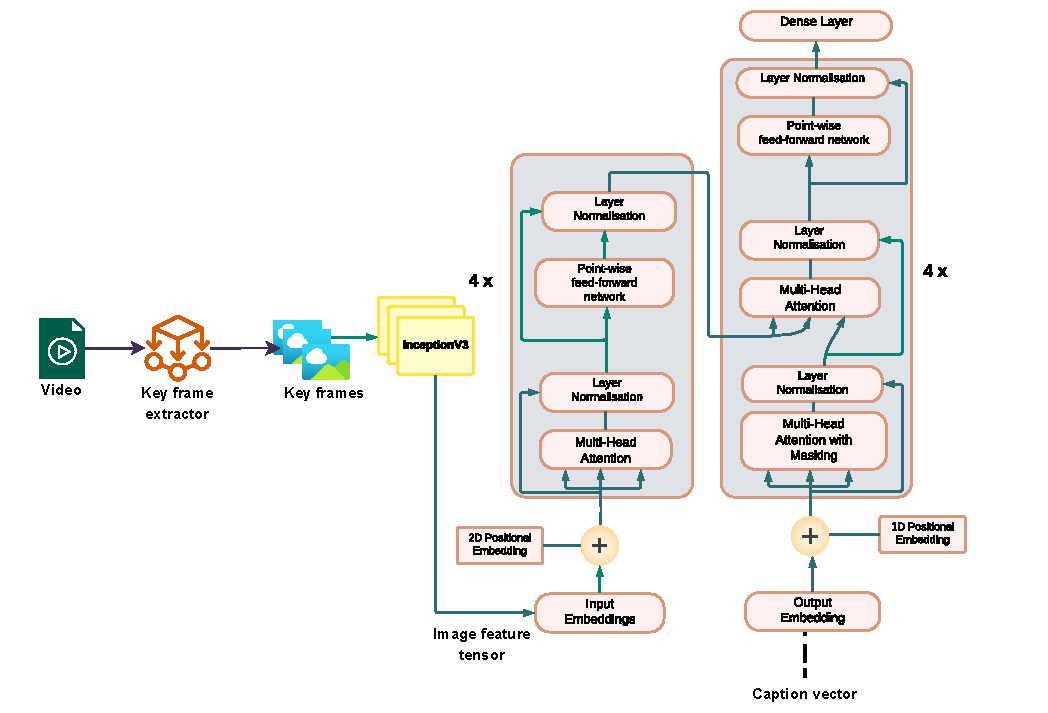
\includegraphics[scale=0.6]{images/baseline.pdf} % set the width to the full text width
  \caption{Our baseline model's architecture, which comprises a video key-frame generator, an image feature extractor, and a vanilla transformer}
  \label{fig:baseline}
\end{figure*} 
As for the transformer architecture, there are 4 encoding and decoding layers with 512 units and 8 attention heads. The size of the feed-forward layer is 2048 and the dropout ratio is set to 0.1. We calculate the attention weights by performing the scaled dot product operation, with masking added to the attention logits before applying the softmax activation function. In the forward pass of the multi-head attention module, the inputs are passed through dense layers and then split into multiple heads. The scaled dot product attention is applied to the bifurcated tensors. The resulting output is transposed, concatenated, and passed through a final fully connected layer. The point-wise feed-forward network is composed of two dense layers, where the first layer has the ReLU activation function applied to its output. In the encoder layer, the input tensor is first passed through a multi-head attention layer with masking, and then a point-wise feed-forward network. Dropout and layer normalisation are applied after each sublayer, and residual connections are added before performing normalisation. Each decoder layer consists of two multi-head attention sub-layers and one point-wise feed-forward sub-layer. The first attention sub-layer applies masked self-attention to the decoder input sequence to prevent attending to future tokens. The second attention sub-layer applies attention to the encoder output and the output of the self-attention layer. The feed-forward layer acts on the output of the second attention. The layers also contains residual connections and layer normalisation for each sub-layer. Additionally, the encoder and decoder contain embedding and positional encoding layers for the image and caption data, respectively. To prevent the decoder from attending to future tokens and to mask out padding tokens in the target sequence, look-ahead and padding masks are created. We use a custom learning rate scheduler that gradually increases the learning rate during the first 5000 steps and gradually decreases it afterwards. Moreover, we use sparse categorical cross entropy loss that effectively masks out the loss over padded values in the input sequence. The loss function returns the average loss per non-padded token in the batch. Finally, the model's parameters are optimised over 20 epochs by applying gradients using the Adam optimiser during the training process.

The implementation is done using Tensorflow with $\approx$ 35M trainable model parameters. The checkpoints are stored and retrieved during evaluation. We evaluate the trained model over images in the test set by first extracting the image features. Then, we feed these features to our transformer to generate captions one word at a time, until the end of sentence token is reached. 

The last step is to processes our video files to extract keyframes. We use OpenCV to read the frames from the video file and then divide each frame into 9 blocks to compute the color histograms. We then apply singular value decomposition to obtain projections of the feature vectors onto a lower-dimensional subspace. Finally, we group the projections and selects keyframes based on a minimum similarity threshold. The keyframes are saved as individual PNG image files which are then captioned using our transformer model. The individual captions are later connected into a paragraph and given as input to ChatGPT to enhance them. Figure \ref{fig:baseline} shows the architecture of our model.

\textbf{Motivation} Is it possible for this simple approach to yield results that are comparable to those of end-to-end models? If not on their own, how do the descriptions generated by ChatGPT compare to the results produced by other models?

\subsection{PDVC}
PDVC \cite{le2021pdvc} is an end-to-end dense framework that uses parallel decoding and directly feeds the intermediate representation into a captioning head, bypassing the two-stage “\textit{localise-then-describe}” scheme. This approach aims to leverage inter-task association at the feature level, allowing the intermediate feature vectors to be matched with target events on a one-to-one basis, making the feature representations more distinct to identify a particular event. It is built upon the "\textit{localise-select-describe}" pipeline, which was first introduced by SDVC, an RNN-based model \cite{Mun2019StreamlinedDV}, to address issues such as caption redundancy, incoherence and the generation of a large volume of proposal-caption pairs. It is scaled to be used in an end-to-end solution that eliminates the need for multi-step training or a recurrent architecture that is often limited in its ability to handle videos with a large number of events.  It is trained on the ActivityNet and YouCook2 datasets.

\textbf{Deformable Transformer} Is a novel architecture whose encoder-decoder structure allows the model to capture the inter-frame, inter-event, and event-frame interactions using its multi-head attention mechanism and produces a set of event query features, which are then used to predict the boundaries and captions simultaneously. This module allows the model to attend to a sparse set of sampling points around reference points and hence mitigates the slow convergence problem of the self-attention mechanism in the Transformer model \cite{Vaswani2017AttentionIA}. It can be formalised as 
\begin{equation}
\mathrm{MSDAtt}(qj, pj, X) = \sum_{l=1}^L \sum_{k=1}^K A_{jlk} W_l X_{pjlk} \phi_l(pj) + \Delta_{pjlk}
\end{equation}
where: $A_{jlk}$ = attention weight between query element $j$ and key element $k$ at scale $l$,
$W_l$ = projection matrix for key elements,
$X_{pjlk}$ = value element at position $(pj,lk)$,
$\phi_l(pj)$ = normalized reference point at scale $l$,
$\Delta_{pjlk}$ = sampling offset at scale $l$. The input is a set of multi-scale feature maps ${X}=\{{x}^l\}_{l=1}^{L}$, a query element $q_j$, and a normalised reference point $\phi_l(p_j) \in [0,1]^2$ while the output is a context vector that contains the weighted sum of $K \times L$ sampling points taken from the feature maps across $L$ scales. K and L are set to 4 while the number of attention heads is 8. The attention dimension is 256 and the size of the feed-forward network is 1024.

\textbf{Feature\,Extraction} We use the R2Plus1D TSP on ActivityNet MaxGVF Backbone architecture \cite{r2plus1d} for determining the frame-level features. The model uses a ResNet-style 3D convolutional neural network (CNN) as the backbone, with temporal segment pooling (TSP) and maximum global video feature (GVF) pooling. The CNN has 34 layers and uses 1x1, 3x3, and 1x1 convolutions in the spatial and temporal dimensions. The TSP operation divides each video into several equal-length segments and pools features within each segment to produce a fixed-length representation of the video. The GVF operation pools features from all segments to produce a single representation of the video. The model is trained using binary cross-entropy loss, with a learning rate of 0.0001 for the backbone and 0.002 for the fully connected layer. The final layer of the model is a fully connected layer with a sigmoid activation function that outputs a probability of the input video belonging to a given activity class. This layer is removed and the pre-trained weights from the remaining layers are loaded into the PDVC model. The feature maps are re-scaled and given as input to the transformer to extract inter-frame relationships.

\textbf{Decoding} Makes use of three types of attention heads. The first of these is the localisation head which utilises a multi-layer perceptron to determine the beginning and end points of an event segment, as well as its confidence score. This is achieved by using the ground-truth segment with a reference center point. The output is the representation of form $ \{t_{s_j}, t_{e_j}, c_{loc_j}\}_{j=1}^N $ for the detected event. While the lightweight captioning head uses an LSTM to predict the next word given an event-level query, the standard captioning head enforces the relationships between words and frames using the deformable soft attention (DSA) module by spanning attention weights over a small area around the reference point. These context features along with the event query features and previous words are concatenated and given to the LSTM and the probability for the next word is obtained by an FC layer with softmax activation. The final component is the event counter that helps find an even balance between tight and sparse sampling of events by max-pooling an event query and subsequently passing it through an FC layer with softmax activation to predict a probability for the possible number of events $r_{len}$ from a global view. During evaluation, the top $N_{set}$ events with accurate boundaries and captions are selected. The confidence score for each event query is calculated using the average of the logarithm of the word probabilities for all the words in the generated caption along with the modulation factors $\gamma$ and $\mu$, to reduce exaggerated confidence for shorter sentences. Finally, the prediction is calculated as the weighted sum of the gIOU, focal and cross-entropy caption losses.

\textbf{Motivation} Can the R2Plus1D TSP backbone architecture provide good captions for our test videos? How closely do the top-\textit{k} descriptions for each frame match the content of the video? Can ChatGPT improve the quality of these descriptions?

\subsection{MART}
MART \cite{liu2020mobile} is a model for video captioning that extends the basic transformer architecture by incorporating a memory-augmented recurrence component. This approach overcomes the limitation of the vanilla transformer to retain extensive sentence and video histories, leading to improved performance in video captioning.
The goal is to generate a coherent video paragraph that describes the content of a video $V$, which consists of multiple event segments $[e_1,e_2,\dots,e_T]$ with sentences $[s_1, s_2, \dots, s_T]$ that describe each event $e_t$ in order.

The video and text embeddings are concatenated $H_0 = [H_{0, \text{video}}; H_{0, \text{text}}]$ and provided as input to MART which has an integrated encoder-decoder architecture. Token type embedding vectors are utilized to distinguish between the embeddings of text and video. The external memory module concatenates the information from its memory states $M^l_{t-1}$ and the intermediate hidden states of the encoder $H^l_{t}$ to update the memory in the current iteration to $M^l_{t}$. Meanwhile, the hidden state representation $H^l_{t}$ is augmented using $M^l_{t-1}$ and passed through a multi-head attention layer before being encoded by the normalisation and residual connection layers inside the transformer block. The model is trained on the ActivityNet and YouCook2 datasets.

\textbf{Motivation}
Before testing MART on our own videos, we train it on ActivityNet captions using a smaller batch size and a reduced number of training epochs. Our aim is to assess whether this approach still produces satisfactory results and if ChatGPT can enhance the quality of the output captions.

\subsection{DenseCap}
DenseCap \cite{johnson2016densecap} is a comprehensive end-to-end model consisting of an encoder, a proposal decoder, and a captioning decoder. It encodes the features of video frames with an encoder, and uses a proposal decoder to determine the start and end timestamps for different proposals by anchoring them. A captioning decoder then decodes the representation specific to the proposal with the help of a masking network. The proposal and captioning decoder are trained consistently using the mask, which allows the proposal module to adjust its prediction based on the quality of the generated caption. It is trained on the ActivityNet and YouCook2 datasets.

\textbf{Video\,Encoder} Encodes each frame of the video $X=\{x_1, \dots, x_T\}$ as a continuous representation $F_0=\{f_{0,1},...,f_{0,T}\}$ and feeds it through 2 encoding layers. Each layer learns a representation of the form 
\begin{equation}
 V(F_l) = \Psi(PF(\Gamma(F_l)),\Gamma(F_l)) 
\end{equation}
where $F_l$ is the input it receives from the previous layer. $\Gamma$ is the representation the self-attention mechanism with 8 attention heads and an attention space of dimension 1024. Each output time-step captures the complete context information by considering a weighted sum of all previous time steps for each query $f_l^t$. The network also includes a 2-layer feed-forward network $PF$ with ReLU activation applied on the first linear layer. Additionally, residual connections and layer normalisation $\Psi$ are applied to both the attention and feed-forward segments. A dropout ratio of 0.2 is used for the attention weights and the residual blocks. The dimension of the feed-forward layer is 2048.

\textbf{Proposal Decoder} The anchor offset mechanism is adapted from ProcNets \cite{Zhou2017TowardsAL}. The event proposal boundaries $(\mathrm{S_p}, \mathrm{E_p})$ are computed using the center and length offsets $\theta_c$ and $\theta_l$, as well as the anchor length $l_a$ and center $c_a$ parameters, respectively. The confidence for each event proposal score is $\mathrm{P_e} \in [0,1]$. The decoder receives the output from the video encoder as its input. It is made up of 3 1D convolutional and batch normalisation layers. ReLU non-linearity is applied at the hidden layer. The kernel size varies from 1 to 251 while the stride factor is set to 50. The stride size varies as a function of the kernel size and stride factor and acts as a preventive measure to avoid long event sequences. 

\textbf{Captioning Decoder} The captioning decoder, as stated earlier makes use of the Masked Transformer to generate natural sentence. For a given word vector $Y^l_{\leq t}$, the 2-layered decoder leverages $\Omega$ to compute the self-attention. It then calculates the element-wise product $\odot$ between the masking function $f_M: \mathbb{R}^{2} \rightarrow [0,1]^T$ over the proposal boundaries and the visual representations $\{F^1 \dots F^l\}$ from the video encoder. The function takes non-zero values near the proposal boundaries and approaches zero elsewhere. More specifically, this masking function prompts the encoder (read video encoder) block of the transformer to regenerate the visual features so as to contain only the information relevant to the current proposal. The masked visual representation from the feed-forward layer of the encoder are then combined with the output of the self-attention layer using $\Psi$ to generate a cross-modal or multi-attention representation, which is then used to predict the probability distribution over the next word in the caption using a linear layer with softmax activation. The final result is thus the probabilities for $w_{t+1}$ which is computed over the product of the word-embedding matrix $W^v$, of vocabulary size $v$ and the decoder output $y_{t+1}$. The dropout ratio is set to 0.2 while the transformer dimension is retained at 1024 units.

\textbf{Differential Proposal Mask} Is the fully differentiable masking function $f_m$ that is computed as a function of 
a parameterised MLP and the logistic sigmoid fuction. This function is especially useful for building the gated mask $f_{GM}$ which is a complementary sum of the output from the proposal decoder and $f_m$ in cases where the confidence score from the proposal decoder is low.

\textbf{Motivation}
We use the pre-trained model's weights on ActivityNet to caption our videos. However, we acknowledge that this approach can lead to repetitive information, especially in long videos where the number of captions can become excessive. Therefore, our goal is to investigate whether ChatGPT can alleviate this issue for us.

\subsection{SwinBERT}
SwinBERT \cite{lin2022swinbert} is a cutting-edge video captioning model that adopts a transformer-based architecture to generate natural language descriptions from video frame patches used as direct inputs. It encodes spatial-temporal representations in a novel way, eliminating the need for multiple computational intensive 2D appearance/3D motion feature extractors which operate on steadily sampled frame rates, as in traditional video captioning methods. Furthermore, this model can handle varying video input lengths with ease. This approach is better than the mainstream sparse sampling method that are commonly used in video-and-language understanding tasks. It is trained on the VATEX, MSRVTT, MSVD, TVC and YouCook2 datasets. It is adept at sampling denser video frames and can thus be relied upon to generate high-quality video captions. The architectural construct is described as follows.

\textbf{Video Swin Transformer} The VidSwin \cite{Liu2021VideoST} model is employed to address the hazard of stacking numerous frames to achieve long-term temporal modeling, which is seminal for effective video understanding. By using the visual encoder with pre-trained Kinetics-600 weights, we can capitalise on its ability to leverage the spatio-temporal locality present in videos, resulting in a balanced trade-off between speed and accuracy. The video frames in their raw form have dimensions of $T \times H \times W \times 3$, where $T$ represents the number of frames and each frame contains $H \times W \times 3$ pixels. The grid features of these frames of dimensions $\frac{T}{2} \times \frac{H}{32} \times \frac{W}{32} \times 8C$, are extracted from the $4^{th}$ and final stage of the Swin transfomer block and dissected 8-ways along the channel dimension $C$, before being sent into the multi-model encoder for caption generation. $T$ is set to 128.

\textbf{Multi-Modal Transformer Encoder} Observes inputs from both caption descriptions and video tokens and performs sequence-to-sequence generation to produce a coherent sentence. The use of a causal self-attention mask allows the encoder to generate output tokens in a uni-directional sense, with each output caption token riveting its focus to its own ground-truth input counterpart. The text tokens are able to access all video tokens, providing additional information about the scene encapsulated by the frames. This allows them to better understand the context of the video and generate more accurate and descriptive captions. Moreover, a trainable sparse attention mask using the sigmoid activation function is employed to regularise the encoder and mitigate issues arising from redundant information in densely sampled consecutive long-input video frames. The dimensions of the attention mask are $(N + M) \times (N + M)$ where $N = 50$ is the length of the textual tokens and $M$ is the size of the single-channel grid features obtained from \textit{VidSwin}. The sparsity constraint \begin{equation}
\mathrm{L_{SPARSE}} = \lambda \cdot M \sum_{i=1}^{M} \sum_{j=1}^{|V_{i,j}|}
\end{equation}
with the regularisation term $\lambda$ and activation values $V_{i,j}$ is used to impose the learnable attention mask $V$ of size $M \times M$ over the video tokens. Over time, the model discovers the most meaningfully rich and high-impact video tokens and forbids connections to inactive tokens with weak correlations.

Moreover, to facilitate the learning of representations that capture the relationship between text and video tokens, a masked language model is used. This involves randomly covering some of the input text tokens using the special token $\mathrm{[MASK]}$, and predicting the most probable value for them based on the surrounding text and video tokens. For generating captions during testing, the model produces one token at a time, taking the previously generated tokens as inputs to the encoder and terminates when the $\langle${eos}$\rangle$ tag is encountered. An MLP is applied to the video tokens to match the sizes of their embeddings with those of the text tokens. The weights are optimised using AdamW \cite{Loshchilov2017DecoupledWD}.

\textbf{Motivation}
Our motivation stems from the following thought – for videos that are extremely long, captioning models may fail due to the need to encode long-term dependencies, which requires structures like memory banks or knowledge graphs to be incorporated \cite{Pan2020SpatioTemporalGF}. Instead of captioning an entire video, what if we are to break them down into \textit{n} partitions, generating individual captions for each of these, and then combining them into a comprehensive description using a large language model like GPT-3? In other words, can ChatGPT effectively decipher the meaning of the video by analyzing the individual captions of each clip despite using such a segmented approach? We partition our test videos into 10-second clips to evaluate our hypothesis.

 VATEX is a vast multilingual video description dataset comprising more than 41,250 videos and 825,000 captions in English and Chinese, including explanations of 600 human activities. Despite SwinBERT not being trained on the ActivityNet dataset, we deem VATEX to be a fitting substitute due to its abundant clip-sentence pairs, extensive lexical content, and similarity to ActivityNet and hence leverage its checkpoints to test our results.

\section{Experiments}
\subsection{Background}
The aim of our experiments was to analyse the qualitative performance of each of the five models and assess the accuracy and coherence of their generated video captions on the ActivityNet dataset. Except for the baseline and MART models, which were compiled and trained from scratch by us, all other models were pre-trained on the same or a similar dataset and had the facility to work with external videos as inputs. The available model checkpoints for DenseCap, PDVC and SwinBERT were retrieved and adapted to generate predictions for each of the videos in our test set. The batch size for the training and validation of MART was set to 16 and 25, respectively, and number of training epochs were limited to 10 as each epoch took approximately 35 minutes to run. It is interesting to note that the ActivityNet-based validation sets for MART and DenseCap had 1471 videos in common. We randomly sampled 26 videos from this set to evaluate our results. DenseCap generated over 300 descriptions for longer videos and had a lot of redundant values for adjacent frames that had to be removed.
The ActivityNet features for these models were pre-compiled and loaded from \cite{dvc}, which used RGB ResNet-200 and Optical flow BN-Inception networks to extract features.

\subsection{Evaluation}
The models generated a collection of one-line captions extracted from or decoded based on keyframes from the videos. These were then submitted as prompts for summarisation to ChatGPT. The idea was to get ChatGPT to provide a human-like summary of the events or activities outlined by the sentences, aiming for an ideal human comprehension of the models' video summarisation outputs. The summaries generated by ChatGPT were compared to the original video descriptions using 4 text evaluation metrics - Cross-Encoder, METEOR, ROUGE and SARI, that best reflected the performance comparisons. For each video, Cross-Encoder, METEOR, and ROUGE required a reference input consisting of the original video description sourced from the ActivityNet captions dataset. This reference was then compared against a hypothesis, which were the ChatGPT-generated summaries in this case. SARI takes into account an additional set of references for a more comprehensive evaluation. We also experimented with other metrics like BLEU, GLEU and SACREBLEU but found their results to be inefficient and unsuitable in accurately representing the difference in model performances.

\textbf{Cross-Encoder} Consists of a transformer network that takes two equal length text inputs and scores their similarity between 0 and 1. Cross-encoders are different from traditional encoder-decoder models used in natural language processing, as they do not generate new embedding but instead focus on comparing and matching existing texts \cite{crossencoder}.

\textbf{METEOR} Is an automatic machine translation evaluation metric which produces a score based on the weighted harmonic mean of unigram precision and recall in the predicted text. It makes use of an alignment algorithm to match ordered words between the candidate and source sentences and computes a unigram match-score between the range of 0 and 1, taking into account textual features such as synonyms and stemming. With its ability to process aspects of context and semantic similarities, it was found to overcome certain limitations of metrics such as BLEU. It also correlates well with human judgments in terms of summarisation quality \cite{meteor}.

\textbf{ROUGE} Is a similar metric that measures the n-gram overlap between the source and reference summaries. It is case-insensitive and also returns a score ranging from 0 to 1, where 1 represents a perfect match \cite{rogue}.

\textbf{SARI} Is a metric used for evaluating the lexical performance of text simplification techniques. By comparing the predicted summary text with the source and reference texts, SARI can evaluate the summarisation model's ability to accurately capture the meaning of the original video descriptions while producing a concise and coherent summary. It produces a score between 0 and 100 that is weighted by the reference text and reflects the goodness of words that were preserved or discarded from the source texts. For our experiments, aside from providing the ground-truth descriptions and the ChatGPT-derived descriptions as the source and prediction texts for this metric, each model's raw output sentences were provided as an extra reference to further guide the evaluation. The purpose of this exercise was to gauge the extent to which machine-generated captions could be comprehended by humans, and to determine the level of similarity between this comprehension and the original events or activities captured in the video sequence \cite{sari}.

\begin{table*}[h]
  \centering
  \resizebox{\linewidth}{!}{%
    \begin{tabular}{ccccccc}
      \includesvg[width=0.8in]{images/v_IlN_XipVf44/frame10.svg} &
      \includesvg[width=0.8in]{images/v_IlN_XipVf44/frame11.svg} &
      \includesvg[width=0.8in]{images/v_IlN_XipVf44/frame12.svg} &
      \includesvg[width=0.8in]{images/v_IlN_XipVf44/frame13.svg} &
      \includesvg[width=0.8in]{images/v_IlN_XipVf44/frame14.svg} &
      \includesvg[width=0.8in]{images/v_IlN_XipVf44/frame15.svg} &
      \includesvg[width=0.8in]{images/v_IlN_XipVf44/frame16.svg}
    \end{tabular}%
  }
    \captionof{figure}{Video ID v\_IlN\_XipVf44 : Shows the video of a man painting a couch}
  \label{sofapainting}
\end{table*}

\begin{table*}[h]
  \centering
  \resizebox{\linewidth}{!}{%
    \begin{tabular}{cccccccccc}
      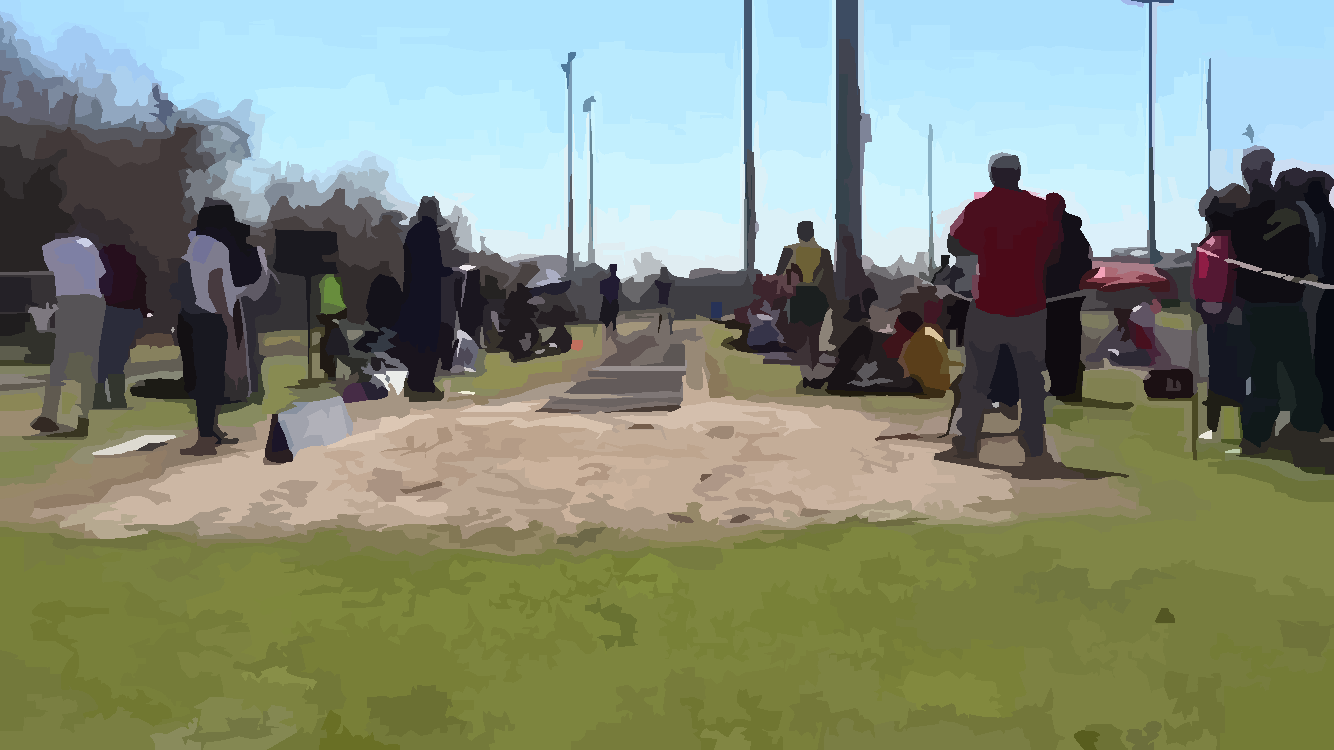
\includegraphics[width=2in, height=1.5in]{images/BCRpdf/frame0.pdf} &
      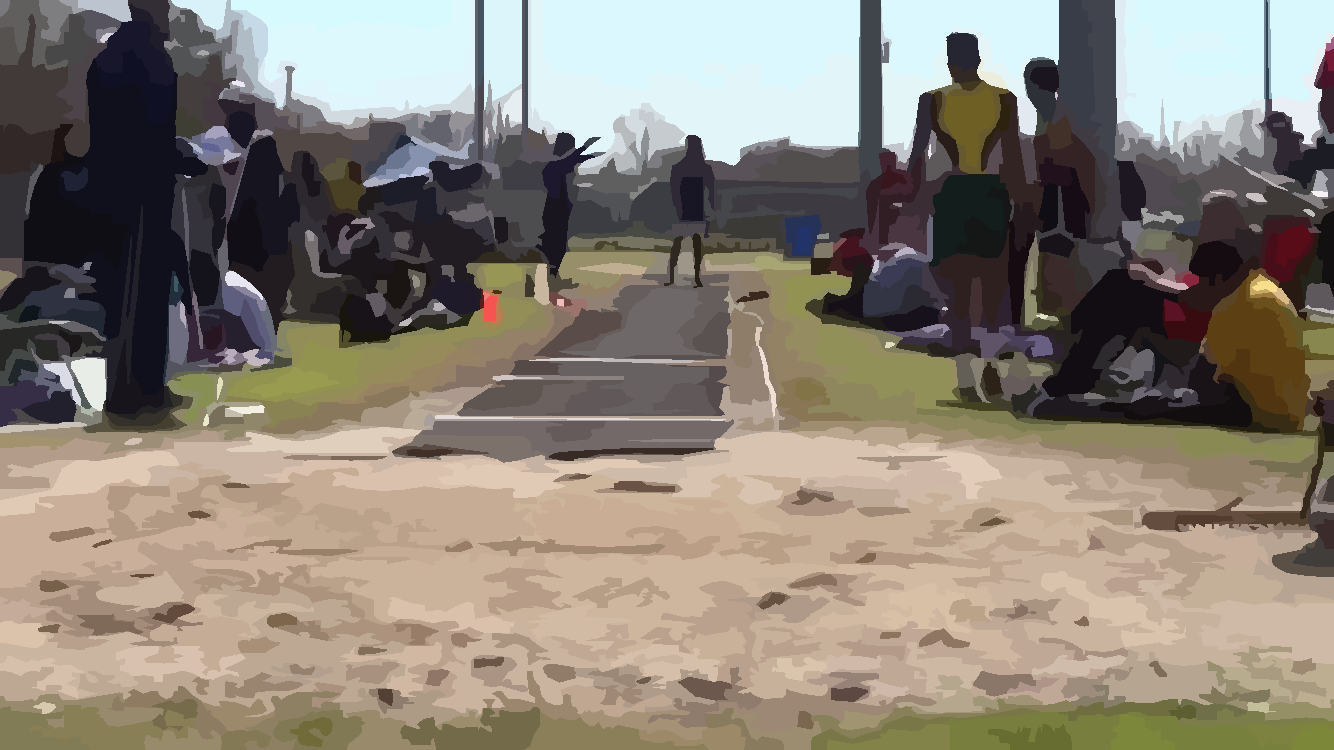
\includegraphics[width=2in, height=1.5in]{images/BCRpdf/frame1.pdf} &
      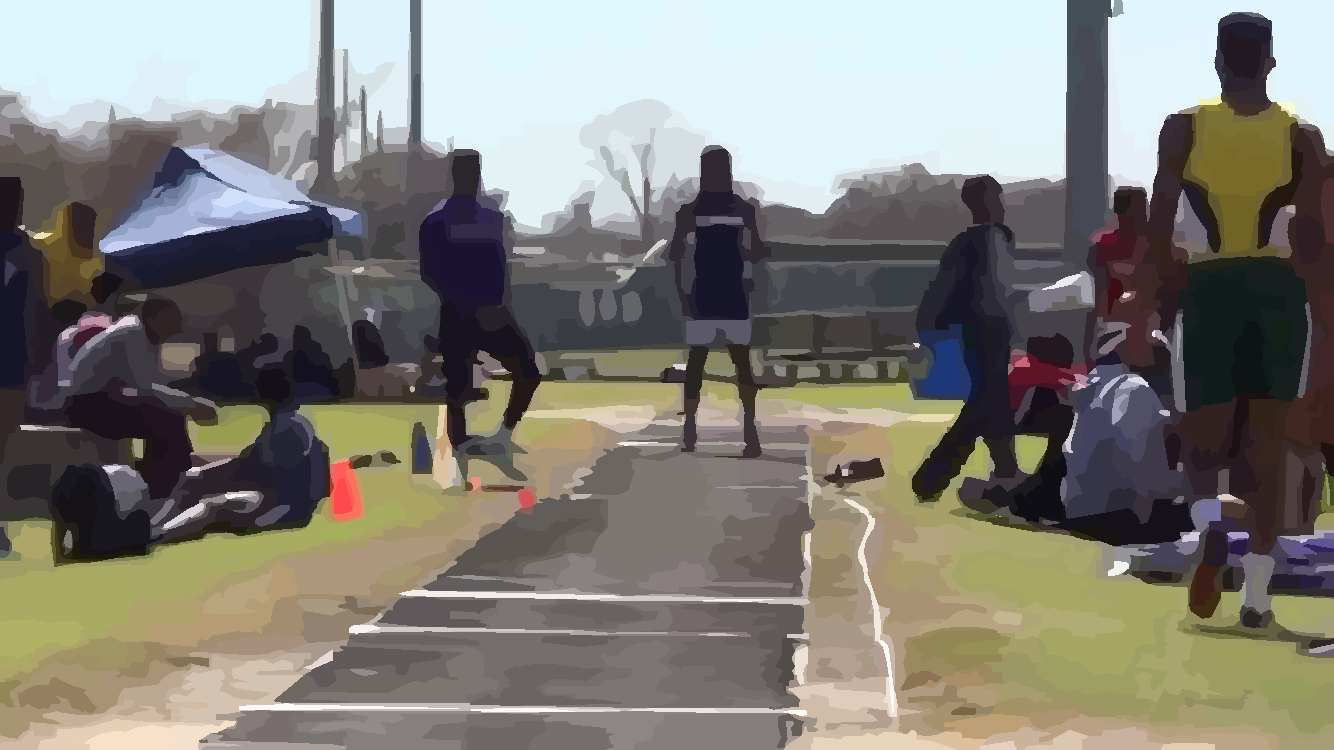
\includegraphics[width=2in, height=1.5in]{images/BCRpdf/frame2.pdf} &
      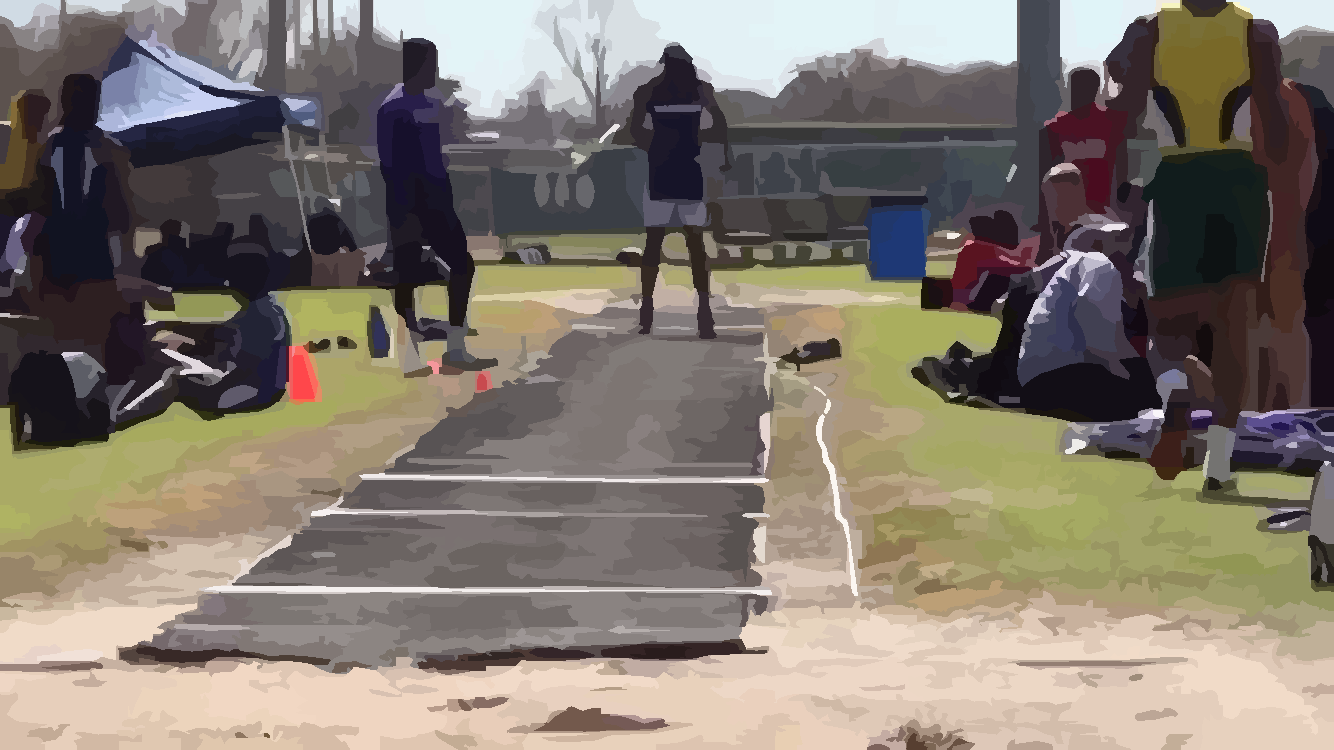
\includegraphics[width=2in, height=1.5in]{images/BCRpdf/frame3.pdf}  &
      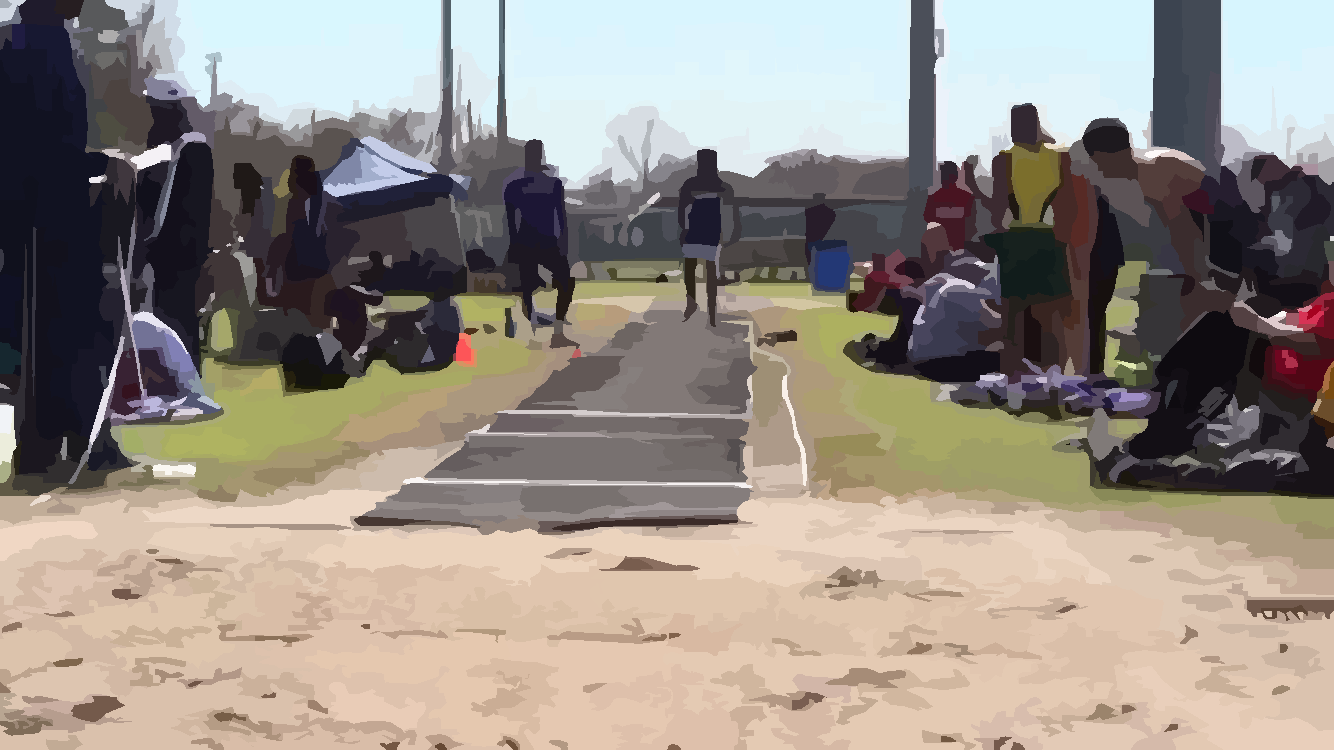
\includegraphics[width=2in, height=1.5in]{images/BCRpdf/frame4.pdf}  &
      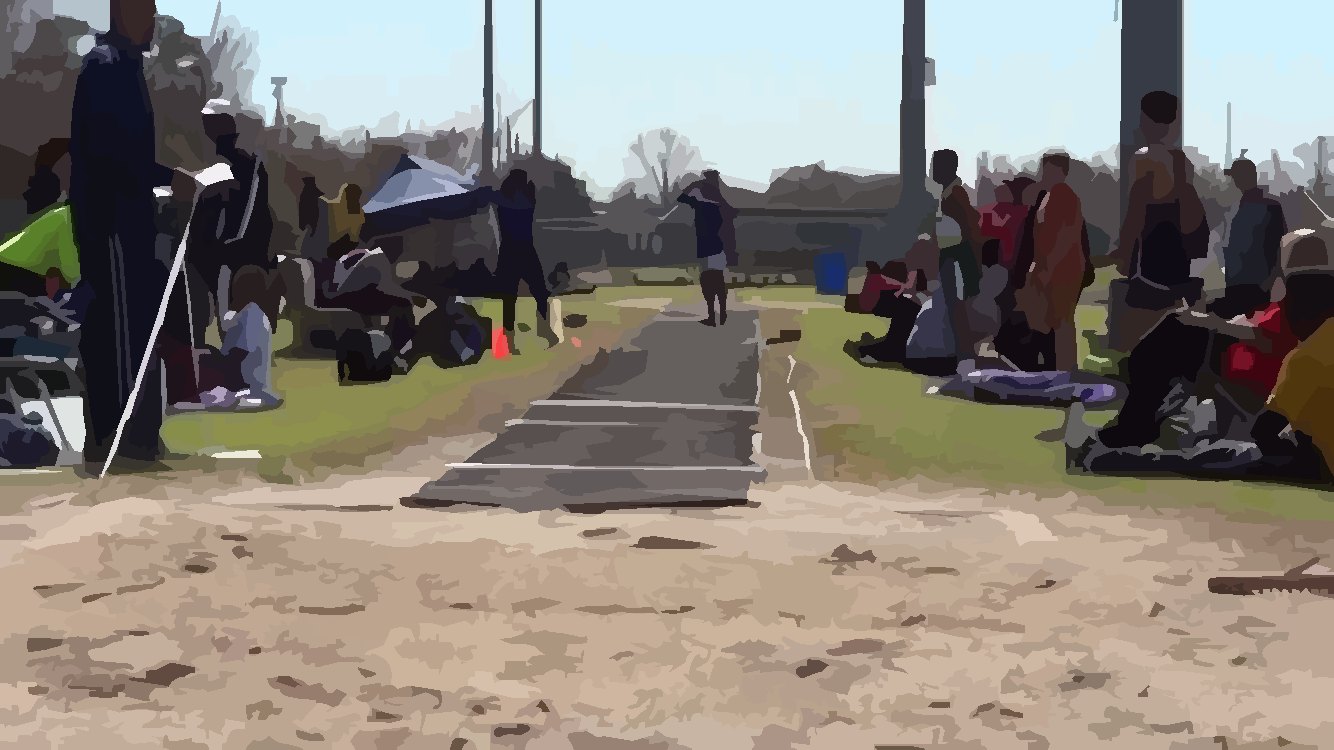
\includegraphics[width=2in, height=1.5in]{images/BCRpdf/frame5.pdf}  &
      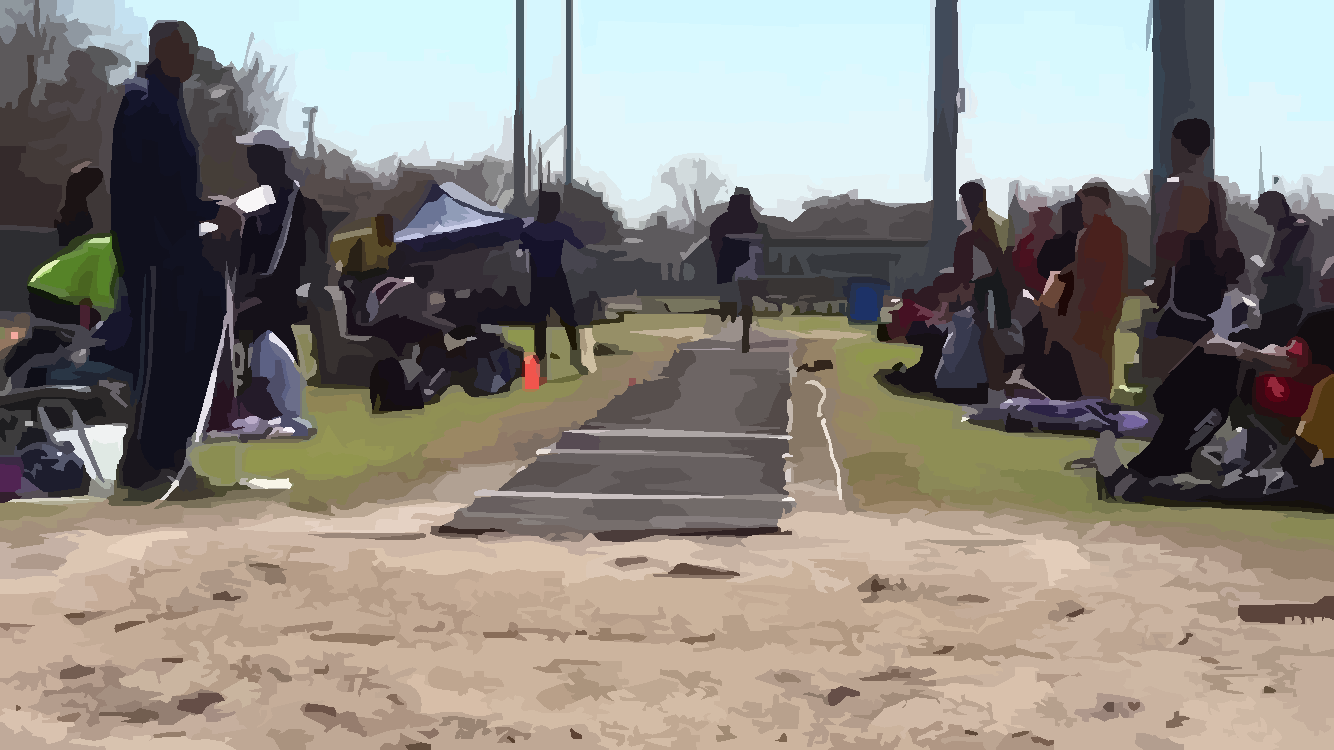
\includegraphics[width=2in, height=1.5in]{images/BCRpdf/frame6.pdf} &
      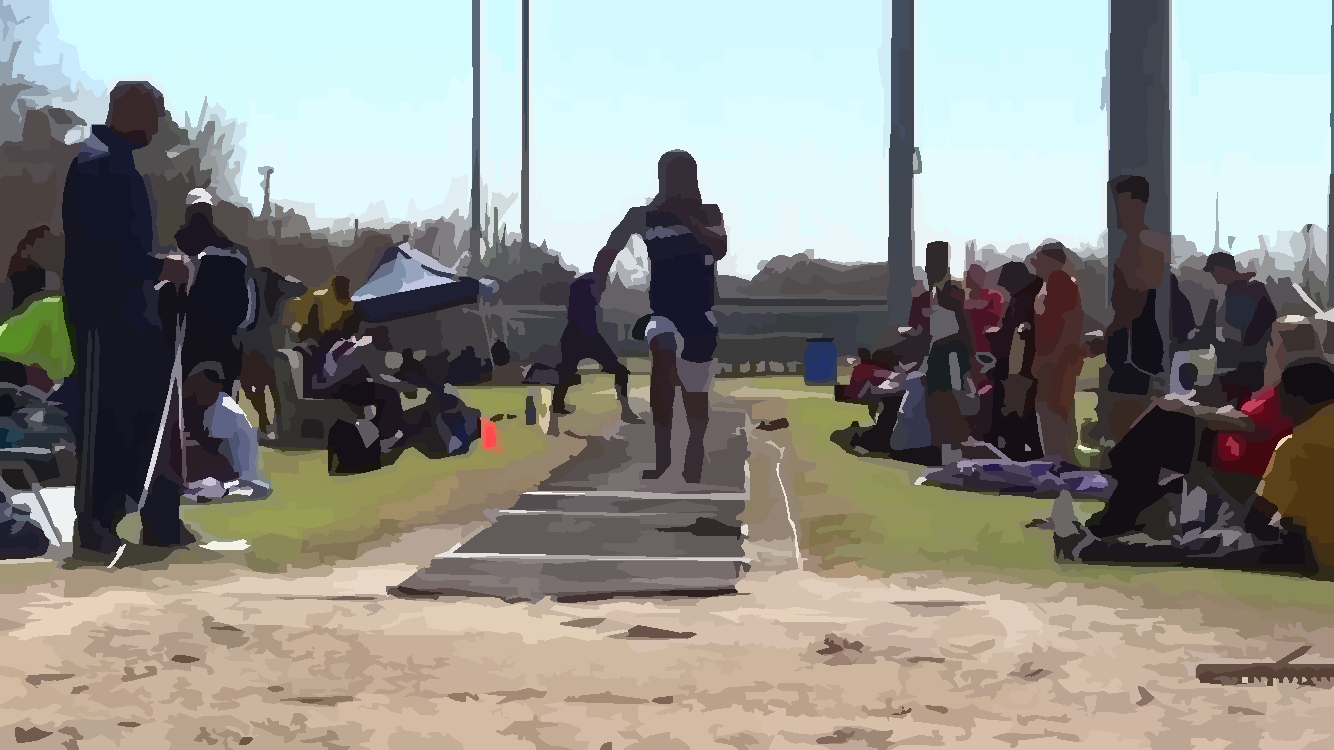
\includegraphics[width=2in, height=1.5in]{images/BCRpdf/frame7.pdf}  &
      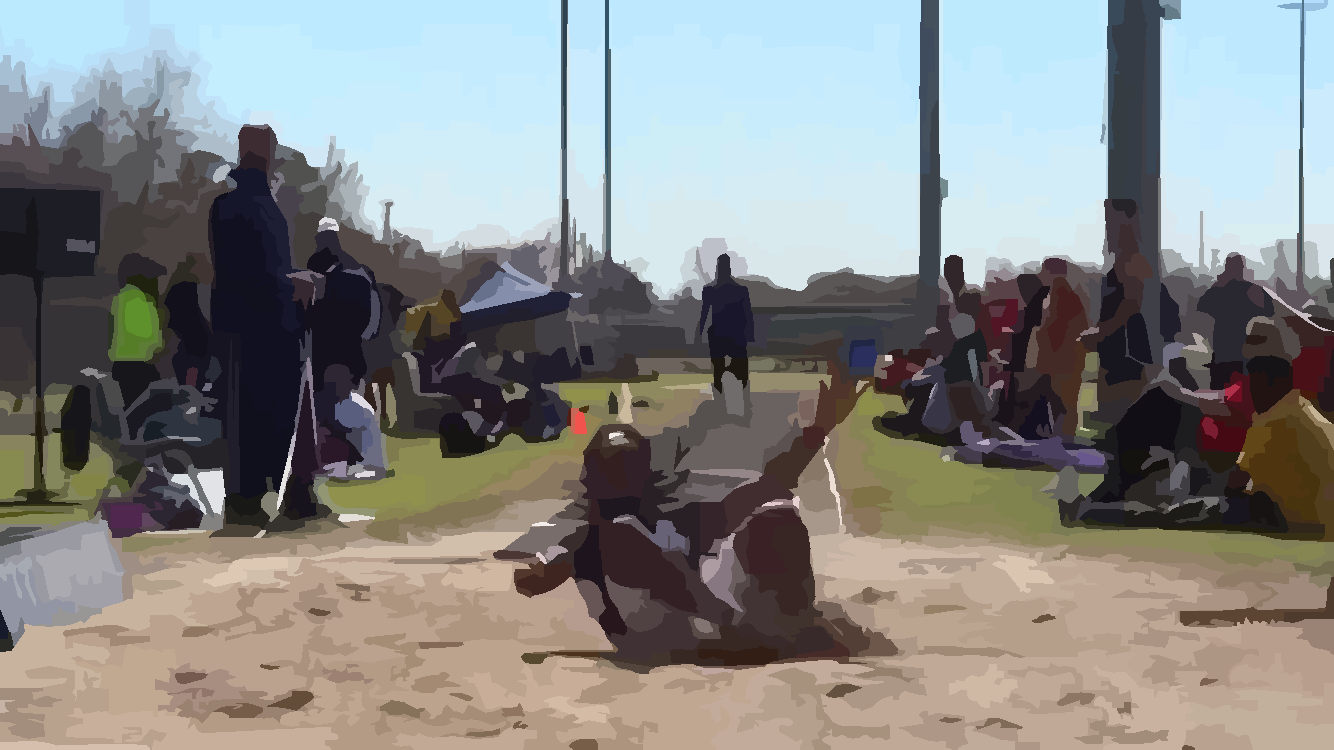
\includegraphics[width=2in, height=1.5in]{images/BCRpdf/frame8.pdf} &
      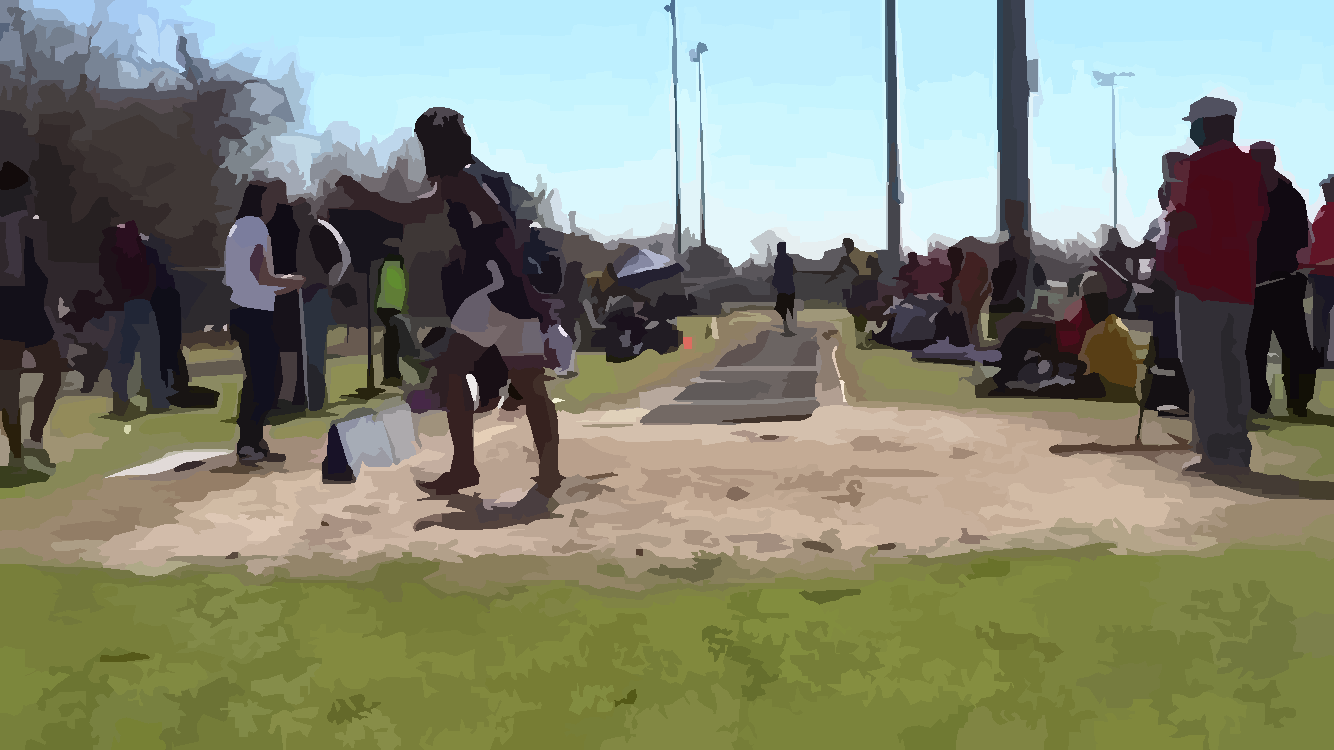
\includegraphics[width=2in, height=1.5in]{images/BCRpdf/frame9.pdf}  \\
    \end{tabular}%
  }
    \captionof{figure}{Video ID v\_BCRFFkvfB\_Q : Shows the video of a man performing a long jump}
    \label{longjump}
\end{table*}

\subsection{Results}
This section interprets and discusses the main findings of our evaluation results. Figures \ref{sofapainting} and \ref{longjump} showcase selected frames from two videos in our test set. Tables \ref{tab:table1} and \ref{tab:table2} and contain their corresponding ChatGPT-generated descriptions obtained using the outputs from each of our tested models. By observing these summaries for accuracy, conciseness, and coherence with the ground truth, we can infer that SwinBERT is likely the best-performing model, followed closely by DenseCap and MART, while our baseline and PDVC models appear to produce inferior quality results.

A closer examination of the evaluation scores listed in Table \ref{tab:table3}, where higher scores indicate better performance, confirms our initial beliefs about the models in general but also reveals new insights about them and the evaluation criteria of the metrics themselves. These values represent the metric score for each model averaged over the scores from all 26 video captions. Higher scores attained by SwinBERT and DenseCap in terms of Cross-Encoders and ROUGE suggest they are better at capturing relationships between the original captions and producing coherent summaries compared to the other models. METEOR scores point towards DenseCap being the most effective at generating summaries that are not only close to the ground truth but also containing a high degree of semantic similarity. As per our expectations, PDVC and the baseline were generally among the worst performing models. Interestingly, the SARI scores did not follow the same trend as the other metrics and revealed some unexpected results. The SARI scores indicate that PDVC performed surprisingly well, while DenseCap and SwinBERT, which performed well on the other metrics and produced more comprehensible summaries, had low scores. This behaviour is visible in Figure \ref{sari-scores}, where PDVC portrays almost contrasting normalized SARI scores for most of the videos against DenseCap, SwinBERT and MART. It is worth noting that SARI evaluates the structural and lexical similarity between the ground-truth and the generated summaries. It is possible that PDVC's summaries had a higher resemblance to the ground-truth values in terms of structure and lexicon, despite being less semantically accurate. Alternatively, it is plausible that SARI may not be equally sensitive to all types of errors or differences between the generated and reference summaries, which could affect the relative rankings of the models. The observed inconsistency may indicate a possible inverse association between SARI scores and model performance. It underscores the significance of using several evaluation metrics to gain a more complete perspective on the models' overall performance. Different metrics measure different aspects of text quality, for instance, ROUGE measures the overlap between generated and reference summaries, while SARI measures the structural similarity between the two. However, the fact that the scores for all the models evaluated are low and ranged closely indicates that no model performed exceptionally well compared to the rest and that there is still room for improvement. It also suggests that the current state-of-the-art models may not be significantly better than simpler baseline models in terms of their ability to generate high-quality summaries. It is possible that these scores were biased by the limited diversity as represented in the 26 videos we evaluated the models upon, or that models such as SwinBERT and DenseCap were unable to adapt to the requirements of the video features, despite being trained on similar datasets.

\begin{figure}[htbp]
\centering
\centerline{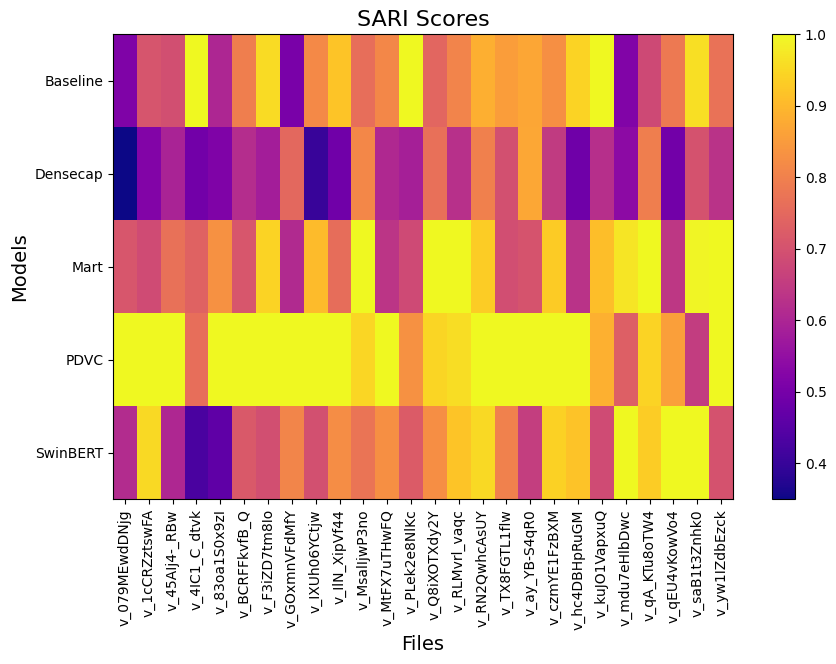
\includegraphics[scale=0.38]{images/sari scores.png}}
\captionsetup{justification=centering}
\caption{Visual representation of the SARI scores of each model on the 26 test videos}
\label{sari-scores}
\end{figure}

\begin{table*}[!htbp]
    \centering
    \renewcommand{\arraystretch}{1.5}
        \begin{tabular}{|p{2cm}p{14cm}|} 
             \hline
             \textbf{Ground Truth} & \textit{Man is in a living room painting a couch with purple spray.
man paint the cushions of the couch on top of paperboard.}\\
             \hline
             \textbf{Baseline}  & A person is seen sitting on a tan chair with a man standing behind them. A young girl is shown climbing a rock wall, and a man is climbing up an icy wall while attached to safety ropes. Another person is sitting inside a room. There's a painting on the wall where a child with a green shirt is sitting. A little boy in blue shorts is seen climbing a bathtub covered in bubbles. Lastly, a man is shown looking down through a window. \\
             \textbf{DesnseCap } & In the video, a woman can be seen kneeling down next to a table and putting a box on the floor. She carefully places a piece of paper into the box and then sets it on the table. She begins to place various objects around the table and in the box, taking care with each item. At one point, she speaks to the camera while kneeling on the floor. After finishing with the objects, she begins to wrap the box in another box, ensuring that it is secure. She then places the wrapped box on the table and starts to clean the floor with a rag. Later, she continues to wrap other boxes while kneeling on the floor and places them on the table. A man is also briefly seen holding a rag and a mop, presumably helping with the cleaning.\\
             \textbf{MART}  &  The video opens with a woman standing in front of the camera, holding a box. She speaks to the camera, explaining something about the box, before placing it on a nearby table. Next, the woman grabs a sheet of paper and puts it on the floor. She takes out some paint and begins to create a colorful pattern on the paper, using a brush. As she paints, she continues to speak to the camera, perhaps discussing her painting process or sharing some thoughts on creativity. The camera captures her movements and the details of her painting as she works. Eventually, she finishes her artwork and holds it up to the camera, showing off her creation. The video ends with the woman thanking the viewer for watching and perhaps inviting them to try their own painting project.\\
             \textbf{PDVC}  & The video starts with a woman speaking to the camera. Then, there is a black screen with white words appearing. After that, the credits of the video are shown several times, followed by a white screen with a white screen appearing, and then a black screen with a white screen appearing again.\\
              \textbf{SwinBERT}  & A man is demonstrating how to use a spray bottle to paint a couch. He holds the spray bottle and applies the paint evenly on the couch, covering every inch of the surface. He shows how to use a smooth, sweeping motion to avoid any uneven patches or drips. The couch gradually transforms from its previous color to a new, vibrant shade. The man takes care to ensure that the paint is applied evenly and covers the entire couch. He completes the process and steps back to admire his work, pleased with the results.\\ 
             \hline
        \end{tabular}
          \caption{Video ID v\_IlN\_XipVf44. Compares the ground truth value for \textit{'Man paintaining a couch'} from ActivityNet with the descriptions obtained from each of our models, after running them through ChatGPT}
    \label{tab:table1}
\end{table*}
\begin{table*}[!htbp]
    \centering
    \renewcommand{\arraystretch}{1.4}
        \begin{tabular}{|p{2cm}p{14cm}|} 
             \hline
             \textbf{Ground Truth} & \textit{A large group of people are seen standing around an area with a man standing in front. The man then begins running down the track with others watching. Finally he jumps into a pit in the end and others measure his throw.}\\
             \hline
              \textbf{Baseline} & A group of people sit on the edge of a march near a grassy body of water, while two others sit in line at the edge of a road, and four men with motorcycles are on a field in a park, while a man skateboards on the ground and people watch, and another man walks on the beach near some rocks, and two people sit in chairs at the park, and a man grinds down a handrail, and skateboard racers jump over a bridge, and two men are on some sand, and two people in brown jackets are running along a rural road. \\
              \textbf{DesnseCap } & A man is standing before a track, ready to take off. His eyes are focused ahead as he takes a deep breath, preparing himself mentally for what's to come. Suddenly, he begins to run down the track, his powerful legs propelling him forward with each step. He moves with a determined stride, his form sleek and athletic as he races towards his goal. Around him, a large group of people watches, their cheers and applause pushing him to go faster and harder. As he reaches the end of the track, he triumphantly raises his arms in the air, a look of satisfaction on his face. He then walks away from the camera, his head held high, knowing he has achieved something great. \\
              \textbf{MART } &  A man is standing on a track and begins walking away. He continues walking and eventually jumps off the ground before walking away from the camera.\\
              \textbf{PDVC}  & Based on the given text, it appears that the video ends with the words on the screen. Throughout the video, there are multiple instances where a woman is seen speaking to the camera, and the credits of the video are shown several times.\\
              \textbf{SwinBERT}  & A man performs a long jump and lands in a sand pit as a few spectators watch him in action.\\ 
             \hline
        \end{tabular}
    \caption{Video ID \- v\_BCRFFkvfB\_Q. Compares the ground truth value for \textit{'Man performing a long jump'} from ActivityNet with the descriptions obtained from each of our models, after running them through ChatGPT}
    \label{tab:table2}
\end{table*}
\begin{table*}[!h]
    \centering
    \renewcommand{\arraystretch}{1.2}
        \begin{tabular}{|p{2.8cm}p{2.3cm}p{2.3cm}p{2.3cm}p{2.3cm}p{2.3cm}|} 
             \hline
             \textbf{Evaluation Metric} & \textbf{Baseline} & \textbf{DesnseCap} & \textbf{MART} & \textbf{PDVC} & \textbf{SwinBERT} \\ 
             \hline\hline
             \textbf{Cross-Encoders} & 0.1537 &  0.2646 & 0.2396 & 0.1329 & 0.3085 \\ 
             \textbf{ROUGE} & 0.1896 & 0.2407 & 0.2439 & 0.1971 & 0.2459\\
             \textbf{METEOR} & 0.1949 & 0.2614 & 0.2510 & 0.1619 & 0.2483\\
             \textbf{SARI} & 63.038 & 48.282 & 64.980 & 74.478 & 61.914 \\
             \hline     
        \end{tabular}
    \caption{Comparison of evaluation metrics for different models}
    \label{tab:table3}
\end{table*}



\section{Conclusions}
\label{sec:concl}
In this study, we evaluated the performance of 5 video captioning algorithms, including a naive baseline model, by using ChatGPT to assess the quality of their generated captions. The evaluation metrics included Cross-Encoders, ROUGE, METEOR, and SARI. While the summaries produced by SwinBERT were found to be the most efficient, the SARI scores revealed some unexpected results. The worst-performing model, PDVC, performed surprisingly well on this metric, while DenseCap and SwinBERT, which performed well on other metrics, scored lower on SARI. Overall, the results suggested that all of the model performances were poor and at par with each other on the ActivityNet dataset, highlighting the need for more challenging evaluations to test their capabilities. One key observation was that splitting videos had a negative impact on the performance of SwinBERT, possibly because the splits were made based on regular time intervals rather than exact event boundaries.

Some possible future directions for the experiments conducted in this project include evaluating other video captioning techniques on the ActivityNet dataset, such as action localisation models that label and localise specific actions or activities in a video at their respective start and end times. Models like BMN and BSN, available in the popular MMAction2 computer vision framework \cite{mmaction}, produce dense feature encodings of the spatio-temporal information in video frames, which can be transformed into captions and coherent video descriptions using any of the transformer-based models we explored. Further studies could also investigate the ethical implications and fairness of the generated video descriptions, which is an important practical aspect to consider in most AI-based applications today. The data used to train the models, evaluation metrics, or ChatGPT's responses may be biased towards certain types of content or languages and could result in inappropriate profiling of individuals or groups in the videos based on their ethnicity, race, religion, or social status. By incorporating such ethical and data protection considerations, the project can contribute to the development of responsible and fair video summarisation techniques that benefit everyone. We also propose to experiment with multi-modal data such as audio to see if this can improve performance. Another natural extension would be to test our results on the recently released GPT-4 model.

\bibliography{example-refs}
\end{document} 

